\begin{figure}[h]
    \centering
    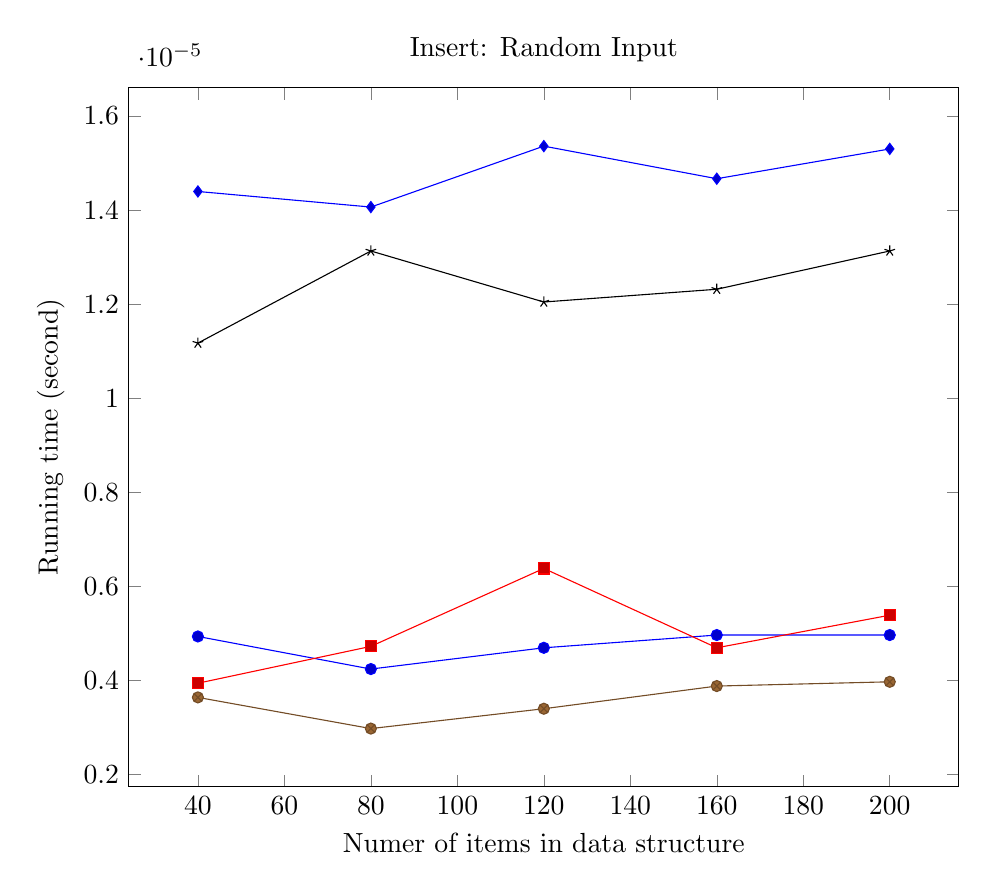
\begin{tikzpicture}
        \begin{axis}[
            xlabel={Numer of items in data structure},
            ylabel={Running time (second)},
            title={Insert: Random Input},
            width=\textwidth
        ]
		\addplot coordinates {
			(200, 4.969393056342142e-06)
			(160, 4.9693930566974135e-06)
			(120, 4.698335253294772e-06)
			(80, 4.246572248334246e-06)
			(40, 4.939275522630737e-06)
		};
		\addplot coordinates {
			(200, 5.391038527946534e-06)
			(160, 4.698335253294772e-06)
			(120, 6.384917139357071e-06)
			(80, 4.728452787006176e-06)
			(40, 3.9453969115754715e-06)
		};
		\addplot coordinates {
			(200, 3.975514445286877e-06)
			(160, 3.885161844152662e-06)
			(120, 3.4032813054807322e-06)
			(80, 2.9816358338763393e-06)
			(40, 3.644221574816697e-06)
		};
		\addplot coordinates {
			(200, 1.3131244682540454e-05)
			(160, 1.2318071273043073e-05)
			(120, 1.2047013469995705e-05)
			(80, 1.3131244682540454e-05)
			(40, 1.1173604993430786e-05)
		};
		\addplot coordinates {
			(200, 1.5299707106919415e-05)
			(160, 1.4667238900045732e-05)
			(120, 1.5359942174342223e-05)
			(80, 1.4064888226172912e-05)
			(40, 1.439618109664309e-05)
		};
        \legend{}
        \end{axis}
    \end{tikzpicture}
    \caption{Average of 0 operations, benchmarked every 0, starting at 0.}
\end{figure}